\documentclass[]{article}
\usepackage{caption,subcaption,graphicx,float,url,amsmath,amssymb,tocloft}
\usepackage[hidelinks]{hyperref}
\usepackage[toc,acronym,nonumberlist]{glossaries}
\setacronymstyle{long-short}
\usepackage{glossaries-extra}
\graphicspath{{figs/}} 

\setlength{\cftsubsecindent}{0em}
\setlength{\cftsecnumwidth}{3em}
\setlength{\cftsubsecnumwidth}{3em}

%opening
\title{
	Notes from Origins of Life\\
	Week 1: Introduction
}
\author{Simon Crase\\simon@greenweaves.nz}

\makeglossaries

\loadglsentries{glossary-entries}

\renewcommand{\thesection}{1.\arabic{section}}
\renewcommand{\glstextformat}[1]{\textbf{\em #1}}

\begin{document}

\maketitle

\begin{abstract}
    These are my notes from the $1^{st}$ week of the Santa Fe Institute Origins of Life Course\cite{sfi2019}. The course aims to push the field of Origins of Life research forward by bringing new and synthetic thinking to the question of how life emerged from an abiotic world.\\
    The content and images contained herein are the intellectual property of the Santa Fe Institute, with the exception of any errors in transcription, which are my own.
    These notes are distributed in the hope that they will be useful,
    but without any warranty, and without even the implied warranty of
     merchantability or fitness for a particular purpose. All feedback is welcome,
    but I don't necessarily undertake to do anything with it.
\end{abstract}

\setcounter{tocdepth}{2}
\tableofcontents


\section{Welcome To The Course}
\begin{itemize}
	\item Dr. Sarah Maurer, Co-creator, video lecturer, and live instructor
	\item Dr. Chris Kempes, Co-creator and video lecture
	\item Maria Kalambokidis, Course materials developer and teaching assistant
	\item Linden Schneider, Online education coordinator and executive producer
	\item Nate Kitchens, Video Editor
\end{itemize}
\section{Life}
Lecturer: David Baum
\subsection{Easy or hard?}
The extremes:
\begin{itemize}
	\item We need to wait billions of years for specific conditions: even hospitable planets lack life--Figure \ref{fig:luca}.
	\item New life can evolve quickly whenever conditions are ripe:  New life could emerge in the lab--Figure \ref{fig:zircons}.
\end{itemize}

\begin{figure}[H]
	\caption{Life is hard: All life we know of traces back to a single 		ancestor--\gls{gls:LUCA}}\label{fig:luca} 
	\includegraphics[width=0.9\textwidth]{Luca}
\end{figure}

\begin{figure}[H]
	\caption{Life emerged quickly: The oldest rocks that could have retained evidence of life do have evidence of life\cite{bell2015potentially}}\label{fig:zircons} 
	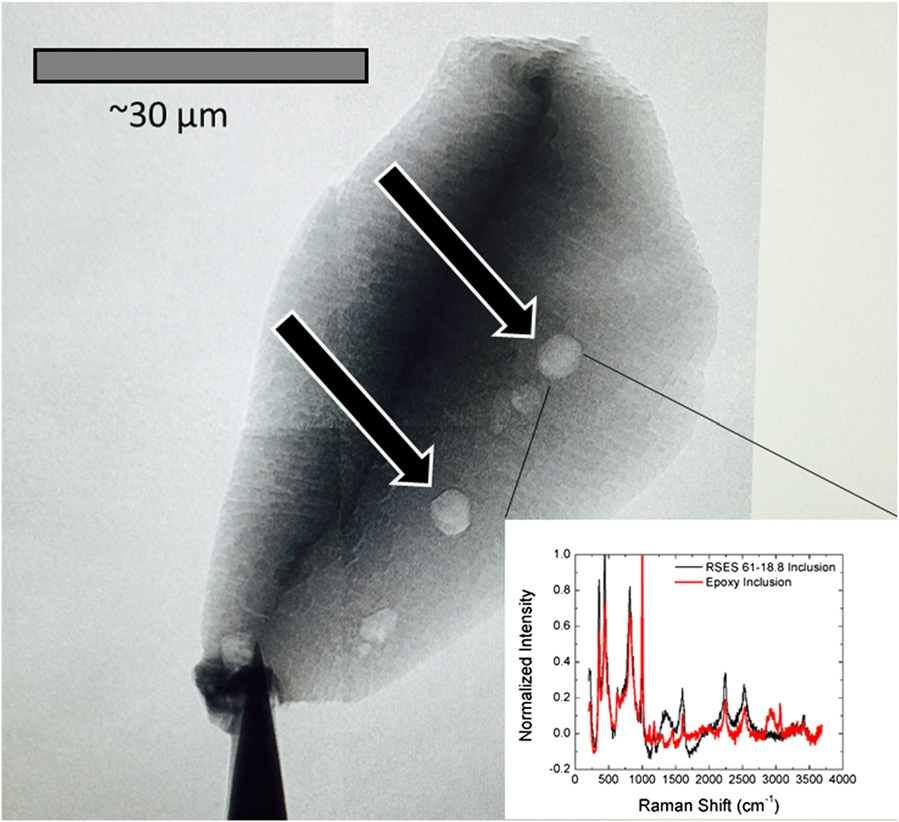
\includegraphics[width=0.9\textwidth]{Zircons}
\end{figure}

\begin{itemize}
	\item Life preempts Life: ''But if (\& oh what a big if) we could conceive in some warm little pond with all sorts of ammonia \& phosphoric salts,—light, heat, electricity \&c present, that a protein compound was chemically formed, ready to undergo still more complex changes, at the present day such matter would be instantly devoured, or absorbed, which would not have been the case before living creatures were formed''--Charles Darwin\cite{darwin1871letter}.
	
	\item Would we recognize alt-life?
	
	\item Some theories allow life to originate easily\cite{wachtershauser1988before}
\end{itemize}

\subsection{The meaning of ''life''}
\gls{gls:LAWKI} shares many features
\begin{itemize}
	\item \gls{gls:DNA}/\gls{gls:RNA} (A,T/U,C, G)
	\item Proteins with the same 20 L amino acids
	\item Genetic Code
	\item Ribosomes
	\item Biochemistry (e.g. \gls{gls:ATP})
	\item Particular genes
\end{itemize}

\begin{figure}[H]
	\caption{\acrfull{gls:LAWKI}}\label{fig:LUCA_figs} 
	
	\begin{subfigure}[b]{0.45\textwidth}
		\centering
		\caption{A reflection of common ancestry}\label{fig:LUCA_common} 
		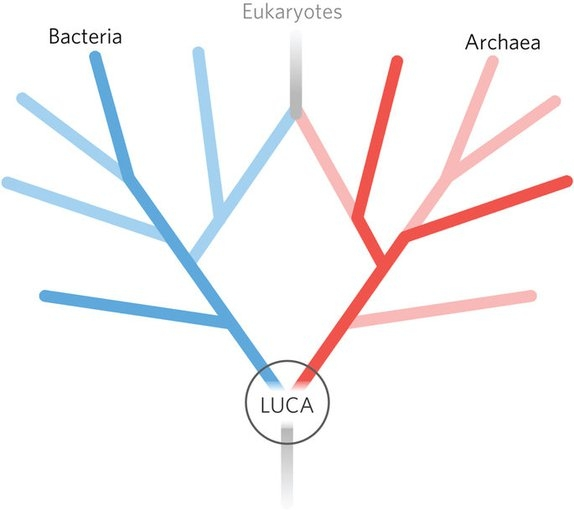
\includegraphics[width=\textwidth]{LUCA_common}
	\end{subfigure}
	\begin{subfigure}[b]{0.45\textwidth}
		\centering
		\caption{Focus on generic features...but which?}\label{fig:lawki-focus} 
		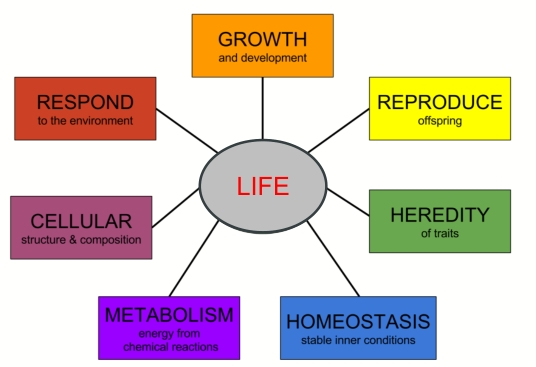
\includegraphics[width=\textwidth]{lawki-focus}
	\end{subfigure}
\end{figure}

\gls{gls:life} is a self-propagating chemical system capable of undergoing adaptive evolution--adapted from \cite{deamer1994origins}
\begin{itemize}
	\item ''Self-propagating'' includes growth and cellular reproduction 
	\item ''Adaptive evolution'' entails the potential to complexify and become more out-of-equilibrium--Figure \ref{fig:AdaptiveEvolution}
	\item Self-propagation and evolution are key
\end{itemize}

\begin{figure}[H]
	\caption{''Adaptive evolution'' entails the potential to complexify and become more out-of-equilibrium}\label{fig:AdaptiveEvolution} 
	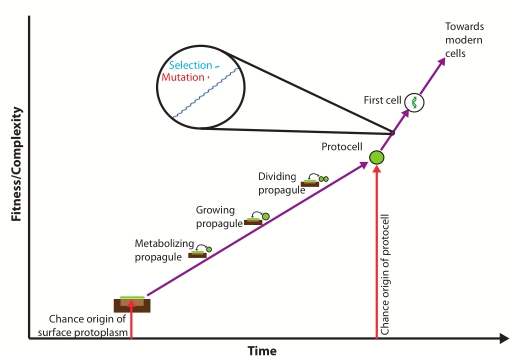
\includegraphics[width=0.9\textwidth]{AdaptiveEvolution}
\end{figure}

\section{Nonequilibrium Physics}

Lecturer: Eric Smith, External Professor, Santa Fe Institute.\\
\\
Topics covered:
\begin{itemize}
	\item The equilibrium concept of phase transition
	
	\item How phase transitions explain robust patterns
	
	\item Why equilibrium isn’t enough to understand life
	\item Phase transitions in dynamical systems ''frozen motion''
\end{itemize}

The ''ordinary'' response of thermodynamic systems to controls. E.g. lava: Viscosity increases smoothly as temperature is lowered. Phase transitions are different
\begin{itemize}
	\item Water does not become harder as it is cooled
	\item It turns to ice suddenly (critical temperature)
	\item The average direction of pointing of the ice sharply increases from zero at the freezing temperature
	\item The direction and strength of the crystal is called the ''Order 	Parameter'' of the transition
	\item Change is sudden because ''you can’t have half a symmetry''
	\begin{itemize}
		\item A direction either exists or it doesn’t
		\item All frozen directions are equivalent
	\end{itemize}
	\item Phase transitions, cooperatively-maintained states, and robustness
	\begin{itemize}
		\item Diamonds are hard because many atoms lock each other in place
		\item The order of the crystal is a ''robust'' property of freezing
	\end{itemize}
\end{itemize}

Evolution happens on a background of robust architectures
\begin{itemize}
	\item Universal small metabolites
	\item RNA and proteins
	\item Cellular and genomic individuality
\end{itemize}

Equilibrium ideas are not enough to explain the robust order of life (Chicken vs. chicken soup)


The Miller-Urey synthesis of amino acids\cite{miller1959organic}

Life is made of interlocking structures and processes: can phase transition ideas
be applied to these?

What might be the order parameters of life?

\begin{itemize}
	\item They would be chemical and energetic
	\item They would involve interdependent	structure and process
\end{itemize}

The characteristic molecules
\begin{itemize}
	\item Unchanging universal roles 	for small metabolites
	\item Key macromolecules such as RNA
\end{itemize}

The great biogeochemical cycles
\begin{itemize}
	\item Life alters cycling of Carbon, Nitrogen, Sulfur, and more
	\item New compounds are also formed of 	these elements
\end{itemize}

\begin{figure}[H]
	\caption{The great biogeochemical cycles\cite{falkowski2008microbial}}\label{fig:biogeochemical} 
	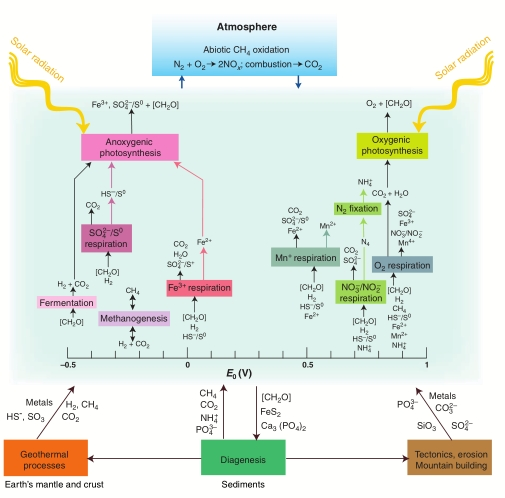
\includegraphics[width=0.9\textwidth]{biogeochemical}
\end{figure}



\begin{figure}[H]
	\caption{Earth’s energy throughput: the Biosphere changes the way a planet converts sunlight into heat.\cite{meadows2005modelling}}\label{fig:EnergyThroughput} 
	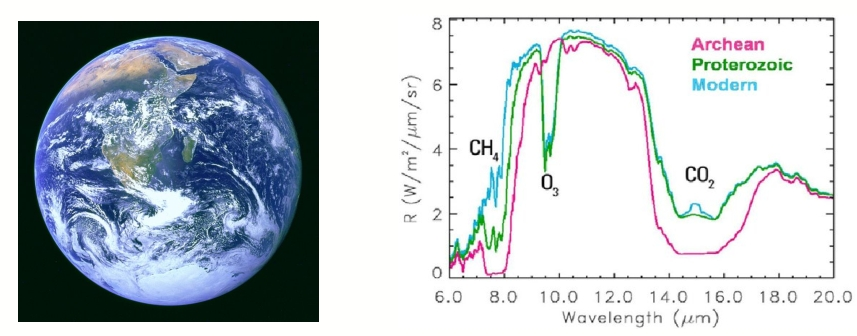
\includegraphics[width=0.9\textwidth]{EnergyThroughput}
\end{figure}

The emergences of individualities
\begin{itemize}
	\item Individuality takes many 	forms
	\item The order parameters in individual-based systems 	are proper names
\end{itemize}

Take-home messages from the lecture:
\begin{itemize}
	\item Phase transitions are one way natural systems  spontaneously form order
	\item The order is robust due to mutual reinforcement
	\item Phase transitions can also lead to spontaneous order in processes like fractures
	\item Candidates for living order parameters include chemical cycles and individuality
\end{itemize}

\section{Constraining Chemical Complexity to Form Life}

Zach Adam
University of Arizona

Most matter isn't live: how to bridge?

\begin{figure}[H]
	\caption{Chemical Complexity}\label{fig:ChemicalComplexity} 
	
	\begin{subfigure}[b]{0.45\textwidth}
		\centering
		\caption{When we first learn chemistry, we use stick and ball model}
		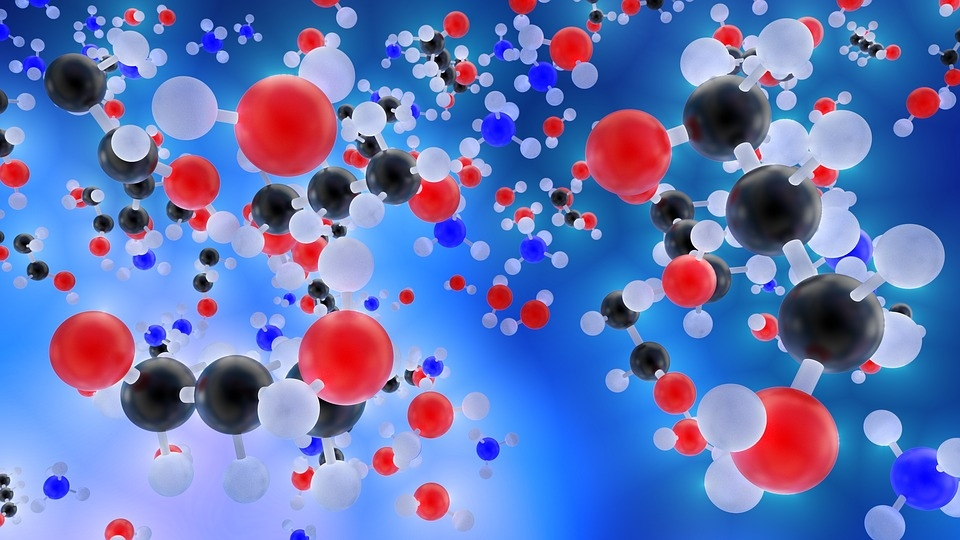
\includegraphics[width=\textwidth]{ChemicalComplexity}
	\end{subfigure}
	\begin{subfigure}[b]{0.45\textwidth}
		\centering
		\caption{But atoms really have many levels, all interacting}
		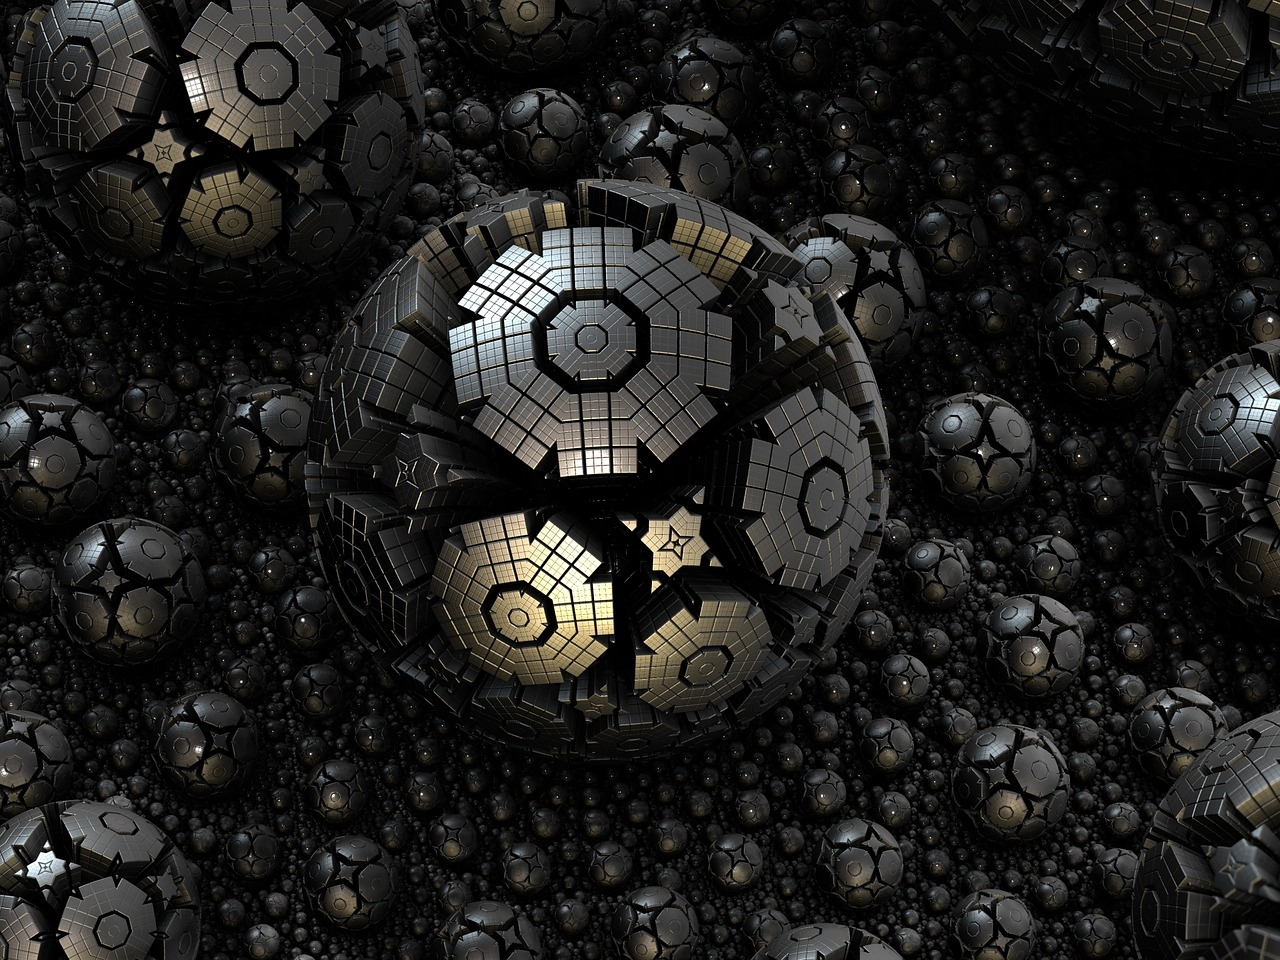
\includegraphics[width=\textwidth]{ChemicalComplexity1}
	\end{subfigure}
\end{figure}


\begin{figure}[H]
	\caption{{Nucleotide Molecule}\label{fig:{NucleotideMolecule} }}
	
	\begin{subfigure}[b]{0.45\textwidth}
		\centering
		\caption{Nucleotide Molecule: one bead expands to 3 molecules. Change one atom, likely to change behaviour of entire molecule!}
		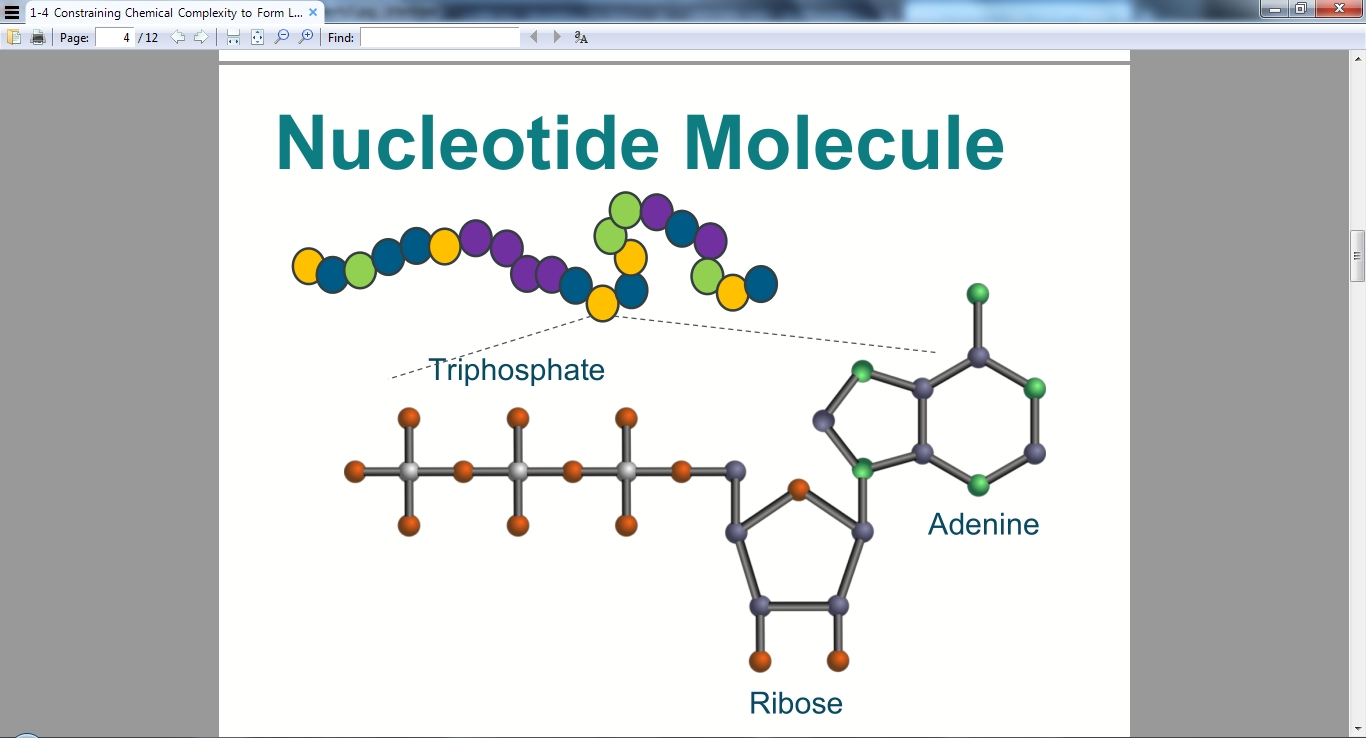
\includegraphics[width=\textwidth]{NucleotideMolecule}
	\end{subfigure}
	\begin{subfigure}[b]{0.45\textwidth}
		\centering
		\caption{Zoom into Adenine Molecule: change one thing, not adenine any more!}
		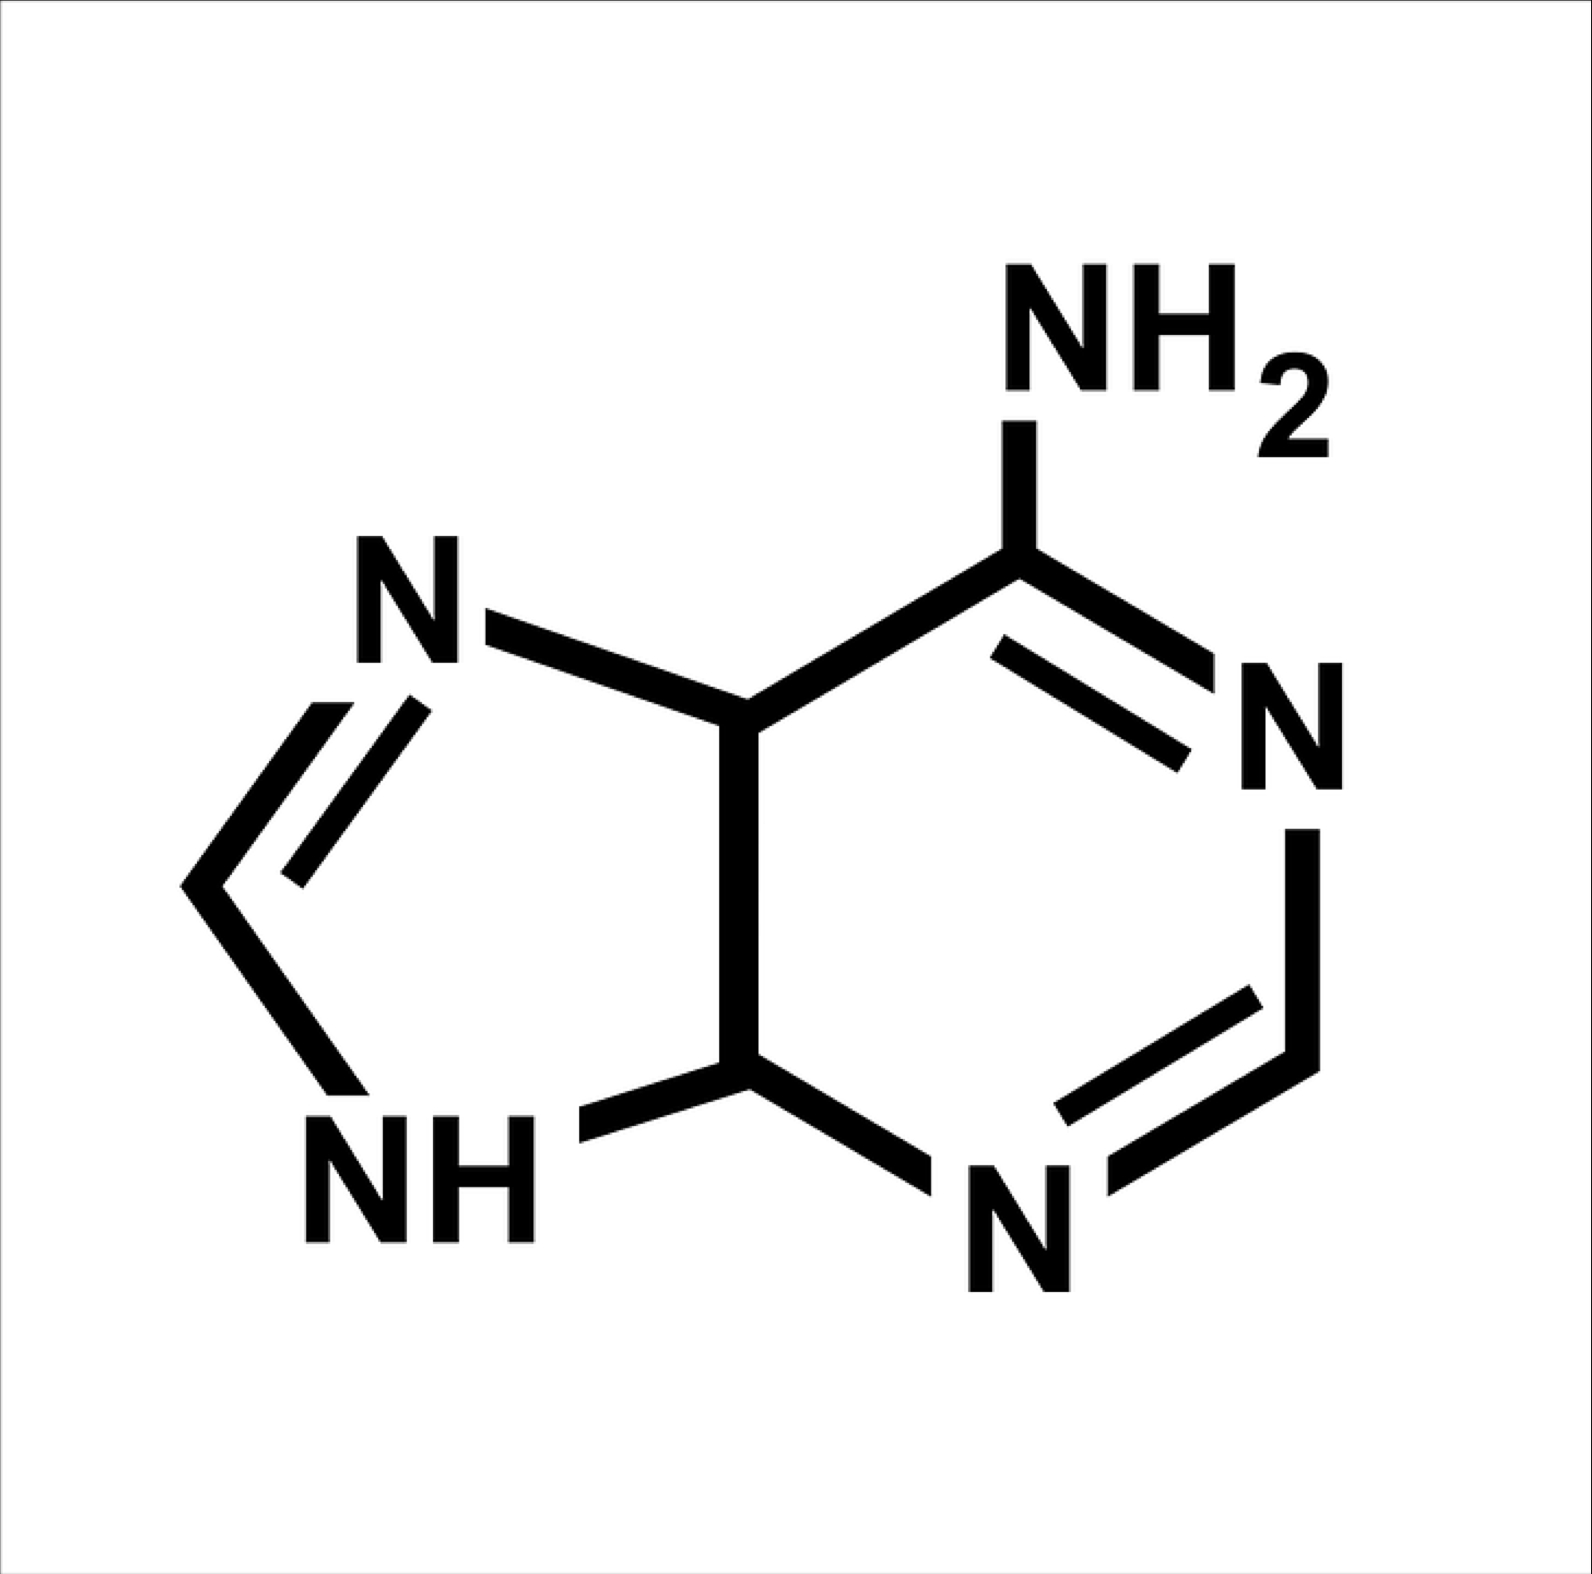
\includegraphics[width=\textwidth]{AdenineMolecule}
	\end{subfigure}
\end{figure}


\begin{figure}[H]
	\caption{Zoom in further, and atoms interact with each other, and with solvents!}\label{fig:MolecularInteractions} 
	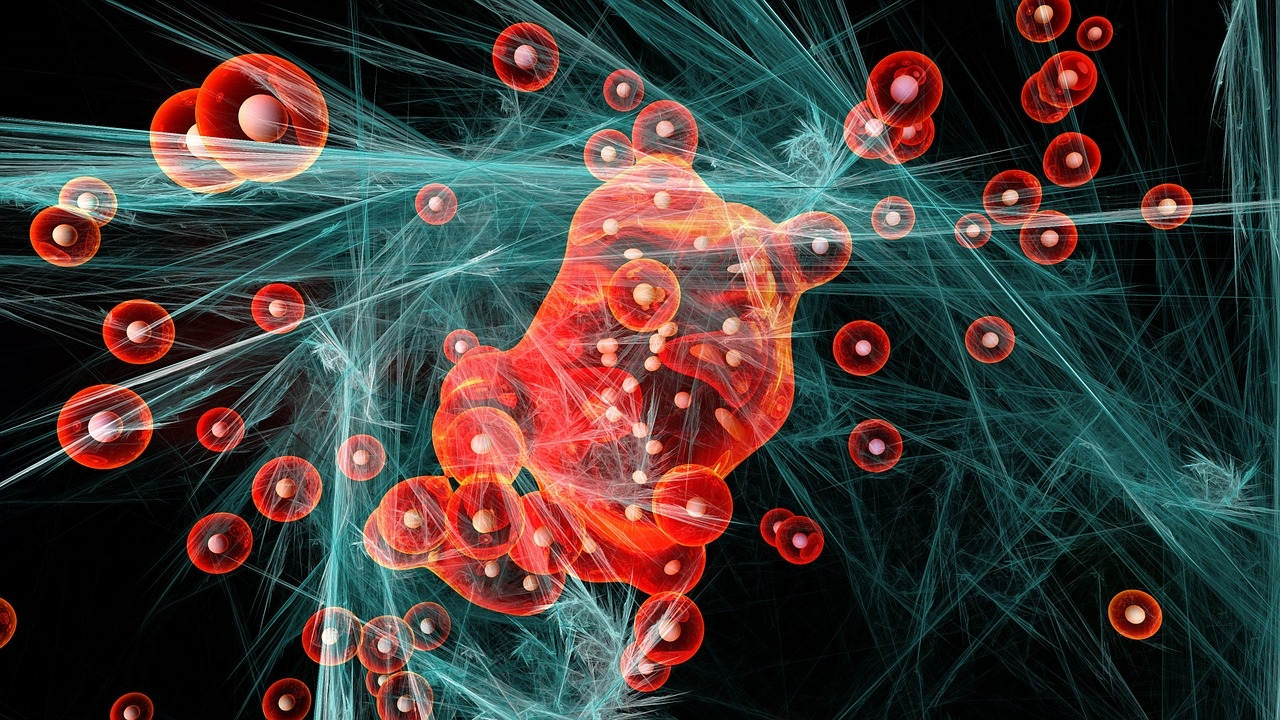
\includegraphics[width=0.9\textwidth]{MolecularInteractions}
\end{figure}

\begin{itemize}
	\item Constrain Location 
	\begin{itemize}
		\item Advantages
		\begin{itemize}
			\item Many possibilities for
			complex interactions
			\item Experiments can be
			designed by analogy
		\end{itemize}
		\item Disadvantages: mostly implausible to
		assume pure reactants in
		natural settings
	\end{itemize}
	\item Constrain Reactants
	\begin{itemize}
		\item Advantages: limit to needed molecules and needed amounts.
		\item Disadvantages: resulting network is not very complex or robust
	\end{itemize}	
	\item Constrain Energy Sources
		\begin{itemize}
		\item Advantages: processes are not location-
		or reactant-specific; many
		outcomes are possible
		\item Disadvantages: Difficult or impossible to
		predict outcomes of
		processes that cross
		multiple object levels
	\end{itemize}
\end{itemize}

Examples
\begin{itemize}
	\item Constrained Location Examples \begin{itemize}
		\item Hydrothermal Vents\cite{martin2006origin}
		\item Atmosphere (Impactor/Shock Synthesis, Lightning,
		Insolation)\cite{chyba1992endogenous} and \cite{miller1959organic}
	\end{itemize}
	\item Constrained Reactant Examples 
	\begin{itemize}
		\item RNA World\cite{powner2009synthesis},
		\item Pyrite-mediated synthesis\cite{wachtershauser1993cradle}
		\item Borate-mediated synthesis\cite{grew2011borate}
	\end{itemize}
	\item Constrained Energy Examples
	\begin{itemize}
		\item \gls{gls:serpentinization}\cite{schrenk2013serpentinization}
		\item Solar flares\cite{airapetian2016prebiotic}
		\item Radioactivity\cite{yi2018radiolytic} and \cite{adam2018estimating}
	\end{itemize}
\end{itemize}
\section{Geological Conditions, Change, and Chaos}

Zach Adam, University of Arizona\cite{spencer2017growth}

What is the source of our understanding of conditions when we thought life originated?
\begin{figure}[H]
	\caption{Earth's Structure: includes everything in Figure, plus minerals, etc. Can only sample surface, plus a few km down.}\label{fig:EarthStructure} 
	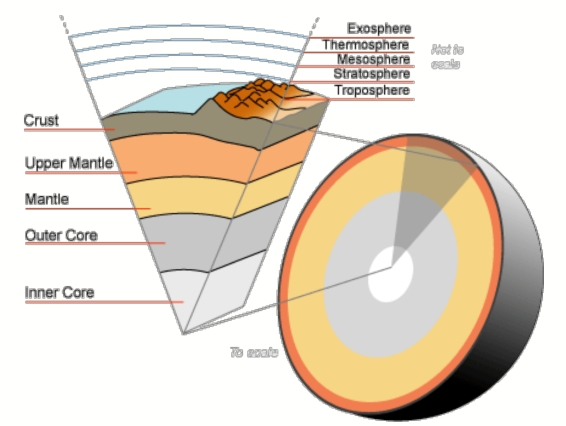
\includegraphics[width=0.9\textwidth]{EarthStructure}
\end{figure}

\begin{figure}[H]
	\caption{Geologic Record is inseparable from history of life}\label{fig:GeologicRecord} 
	
	\begin{subfigure}[b]{0.45\textwidth}
		\centering
		\caption{Great oxidation event changed all sorts of stuff. We need oxygen, but other critters had to adapt or die. Oxidation changed minerals.}
		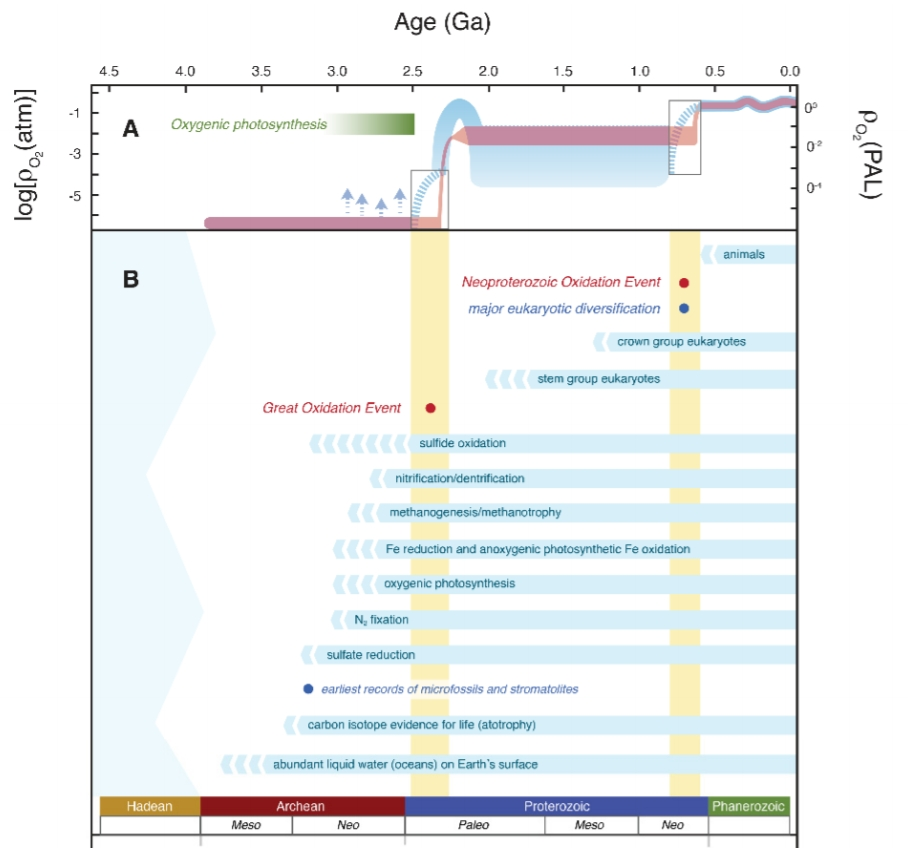
\includegraphics[width=\textwidth]{GeologicRecord}
	\end{subfigure}
	\begin{subfigure}[b]{0.45\textwidth}
		\centering
		\caption{Different models for crustal accumulation.}
		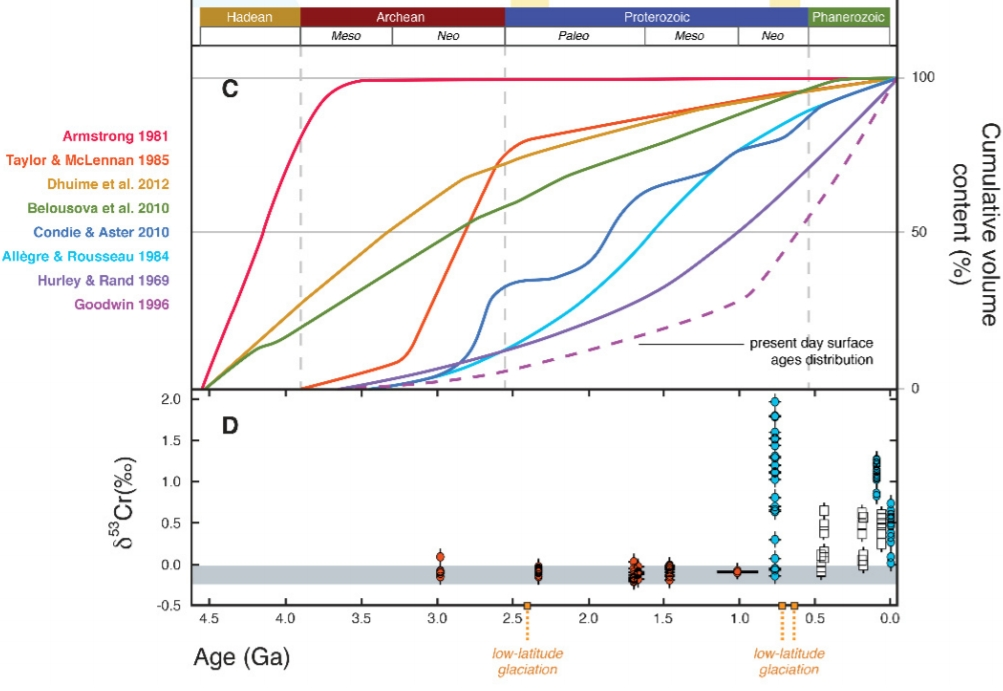
\includegraphics[width=\textwidth]{GeologicRecord1}
	\end{subfigure}
\end{figure}

\begin{figure}[H]
	\caption{Another Level Down: different models for accumulation of crust. Not simple accumulation!}\label{fig:AnotherLevelDown} 
	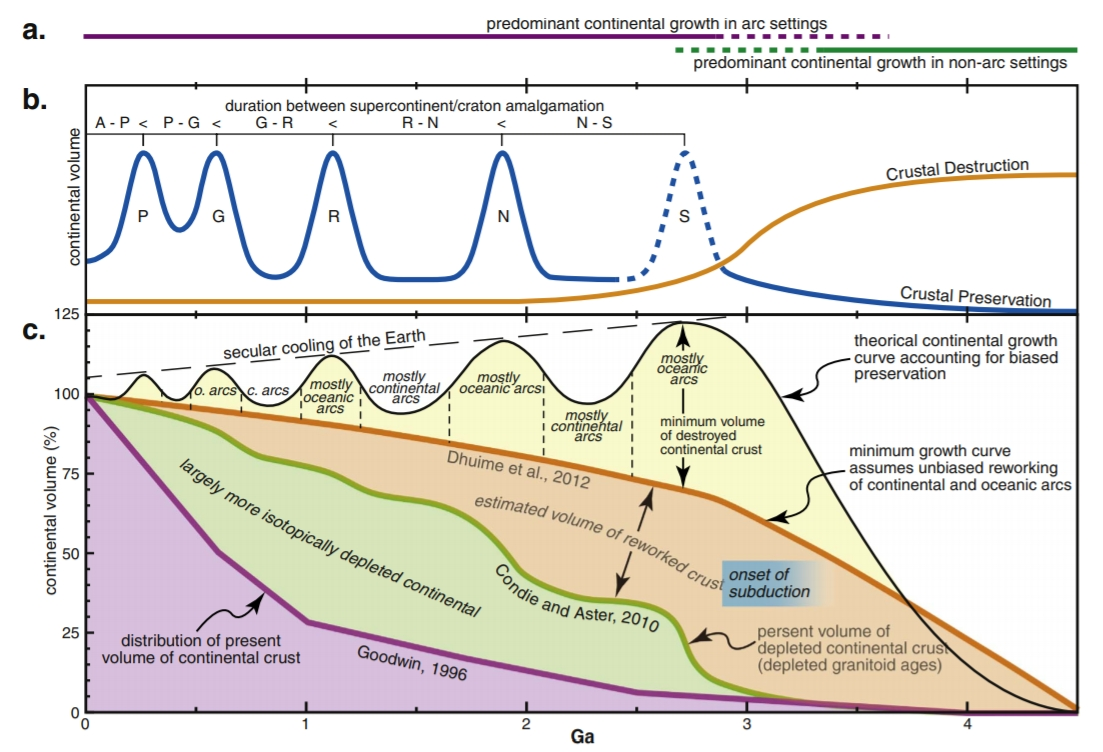
\includegraphics[width=0.9\textwidth]{AnotherLevelDown}
\end{figure}

Only direct record for events that sow chaos and processes of prolonged gradual change

What does this mean for origins of life research?
\begin{itemize}
	\item Limited direct rock data
	\begin{itemize}
		\item 	Sampling and preservation
		biases abound!
			\item No rock packages to
		provide environmental
		context or views into surface
		conditions.
		\item 	No rocks and few minerals
		from time surrounding life’s
		origins.
	\end{itemize}
	\item Complementary lab data
	\begin{itemize}
		\item Experiments are critical for
		filling in where the rock
		record is not available.
			\item Unclear whether powerful
		events/energy are more
		constructive than destructive.
	\end{itemize}
\end{itemize}
\section{Pattern Formation in Chemical Systems}
Chris Kempes

\begin{itemize}
	\item What properties and processes are easy to obtain through physical dynamics alone?
	
	\item How might this make it easy for lifelike things to begin?
	
	\item Reaction Diffusion Equations\cite{sfi_grayscott2018}
\end{itemize}

Describe reaction of $U$ everywhere in space.
\begin{align*}
\frac{\partial U}{\partial t} =&   \underbrace{\overbrace{D_V}^\text{diffusivity} \underbrace{ \nabla^2 U }_\text{difference in fluxes}}_\text{diffusion term} + \underbrace{ F(U)}_\text{reaction term}
\end{align*}

With two chemicals...
\begin{align*}
\frac{\partial U}{\partial t} =&   D_U \nabla^2 U + F(U,V)\\
\frac{\partial V}{\partial t} =&   D_V \nabla^2 V + G(U,V)
\end{align*}

Consider two reacting species, $U$ and $V$, and an inert product $P$.
\begin{align*}
U + 2V \Longrightarrow& 3V\\
V \Longrightarrow& P\\
\frac{\partial U}{\partial t} =& -U V^2 + \overbrace{F}^\text{Fixed flow into system (chemostat)} (1 - U) + D_u \nabla^2 U \\
\frac{\partial V}{\partial t} =& U V^2 - (F +\underbrace{f}_\text{loss to make $P$}) V + D_v \nabla^2 V 
\end{align*}

\begin{figure}[H]
	\caption{Grey Scott Reaction}
	
	\begin{subfigure}[b]{0.45\textwidth}
		\centering
		\caption{Starting configuration}
		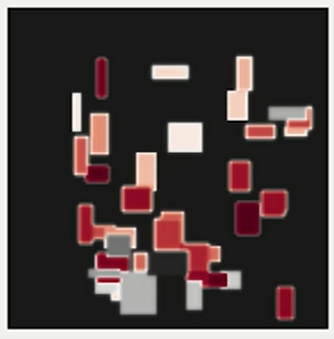
\includegraphics[width=\textwidth]{GreyScottInitial}
	\end{subfigure}
	\begin{subfigure}[b]{0.45\textwidth}
		\centering
		\caption{Evolves toward steady state,  where high concentration close to low concentration. Segregation.}
		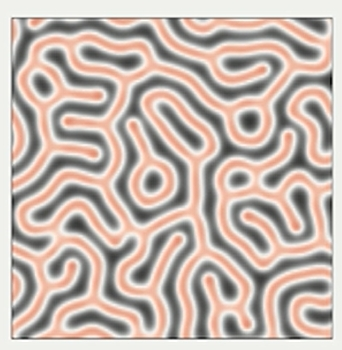
\includegraphics[width=\textwidth]{GreyScottFinal}
	\end{subfigure}
\end{figure}

Other starting values give cell-like behaviour (including division), so maybe get some ''lifelike" behaviour from physics and simple chemistry.

\section{The Central Dogma of Biology}


\subsection{The Central Dogma of Biology}

How do we unwind present day life to learn about origins? Focus on most common properties of all life, especially the Central Dogma.\cite{crick1958biological} \cite{crick1970central}

\begin{figure}[H]
	\caption{The Central Dogma after \cite{crick1970central}}\label{fig:CentralDogma} 
	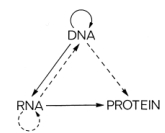
\includegraphics[width=0.9\textwidth]{CentralDogma}
\end{figure}


\begin{figure}[H]
	\caption{Ribosome is conserved across life, but appears to have onion structure, built up by evolution. Ribosome started with common core, and more added.\cite{hsiao2009peeling}.}\label{fig:Ribosome} 
	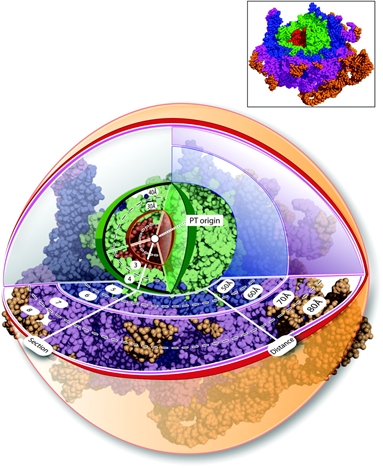
\includegraphics[width=0.9\textwidth]{Ribosome}
\end{figure}
Williams argues that we can use the onion, Figure \ref{fig:Ribosome}, to unwind evolution.

\begin{figure}[H]
	\caption{Ribosome Phases after \cite{petrov2015history}}\label{fig:RibosomePhases} 
	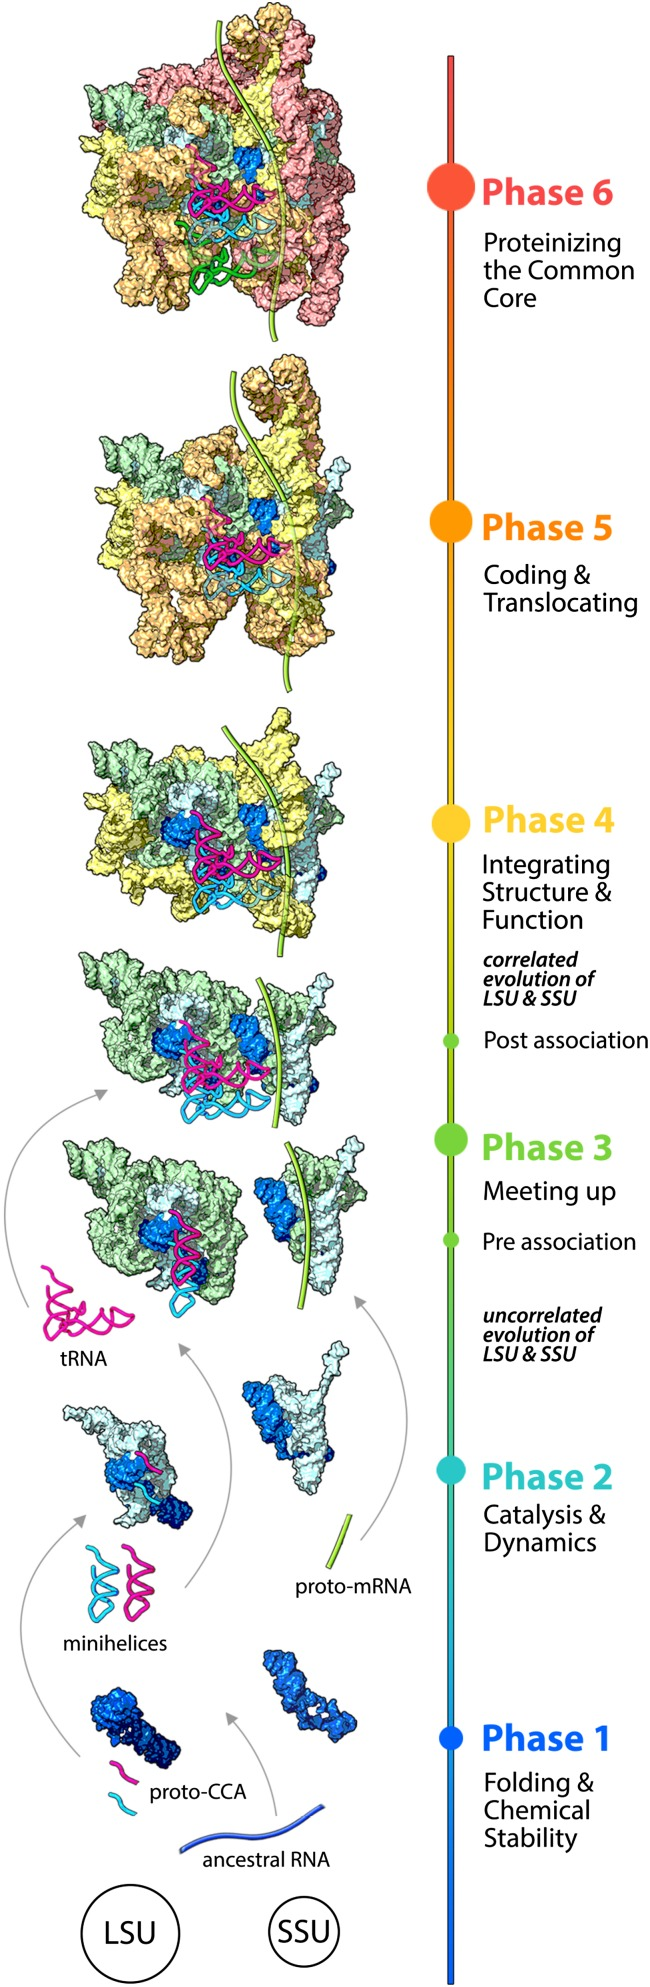
\includegraphics[width=0.5\textwidth]{RibosomePhases}
\end{figure}

Carl Woese used this to build new Tree of Life.

\begin{figure}[H]
	\caption{\gls{gls:TOL}}\label{fig:TOL} 
	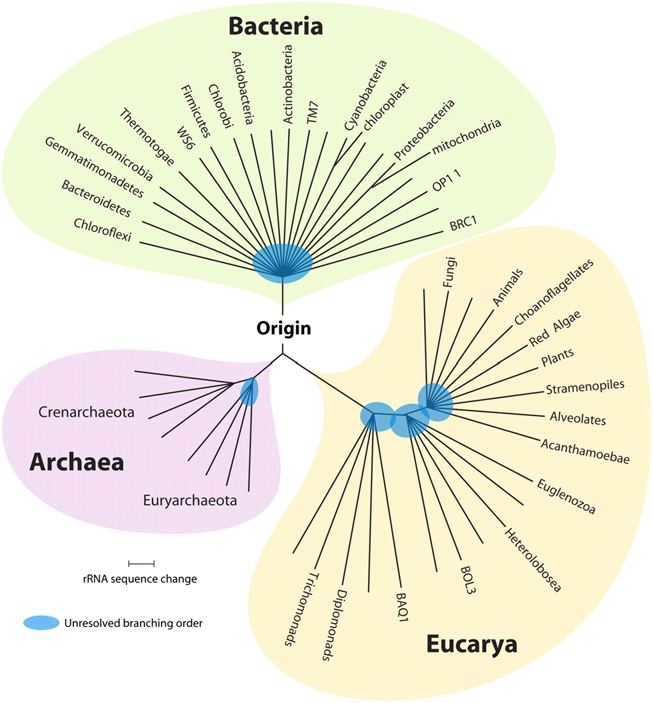
\includegraphics[width=0.9\textwidth]{TOL}
\end{figure}



\subsection{The Efficiency of the Central Dogma of Biology}

Landauer Bound: ''any logically irreversible manipulation of information, such as the erasure of a bit or the merging of two computation paths, must be accompanied by a corresponding entropy increase in non-information-bearing degrees of freedom of the information-processing apparatus or its environment''--$kT(H_i - H_f)$, where $H_i$ represents the entropy of the initial state, $H_i$ of the final\cite{wiki:landauer}\cite{bennett2003notes}\cite{landauer1961irreversibility}. 

\begin{figure}[H]
	\caption{Take unordered set of letters and try to write as specific string.}\label{fig:LandauerRibosome} 
	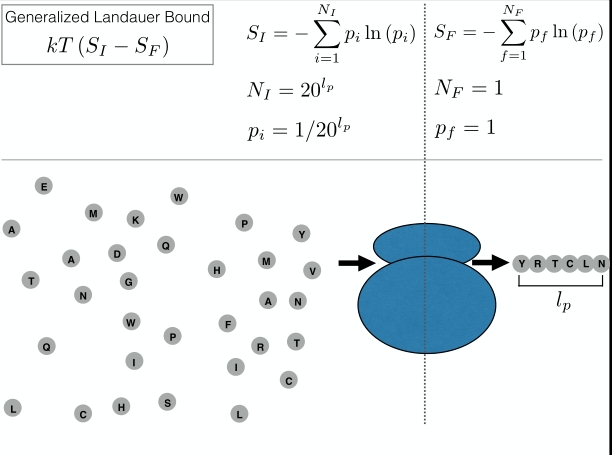
\includegraphics[width=0.9\textwidth]{LandauerRibosome}
\end{figure}

\begin{itemize}
	\item Life is only 20 times less efficient that physical limit\cite{kempes2017thermodynamic}
	\item Computers are 20 times worse than Landauer's bound!
\end{itemize}

\begin{figure}[H]
	\caption{For small cell, \gls{gls:DNA} and proteins take up (nearly) entire volume; for large cells, Ribosome does same thing! So we have bounds on allowable volume.\cite{kempes2016evolutionary}}\label{fig:RibosomeTradeoffs} 
	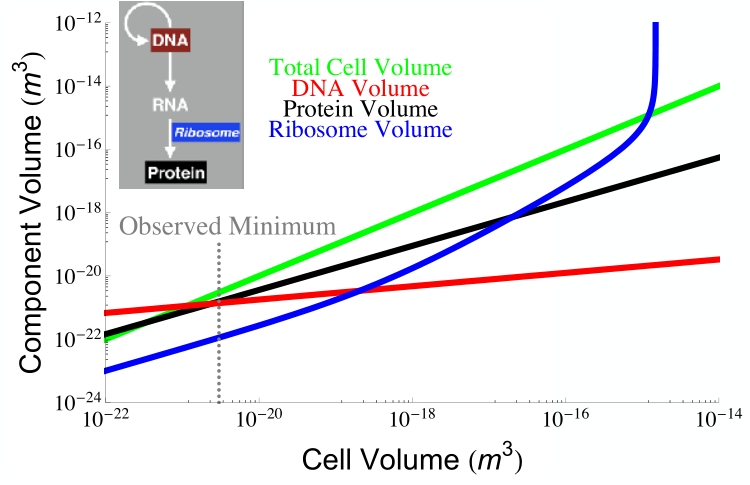
\includegraphics[width=0.9\textwidth]{RibosomeTradeoffs}
\end{figure}

\begin{figure}[H]
	\caption{A more efficient ribosome would allow larger cells; less efficient might not work at all.}\label{fig:RibosomeTradeoffsEarly} 
	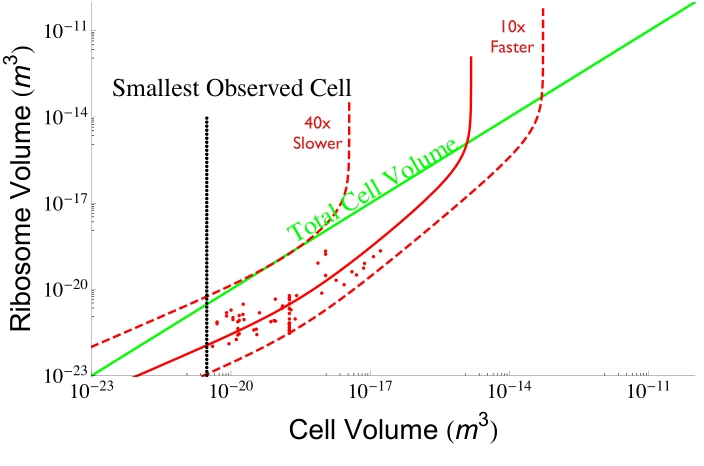
\includegraphics[width=0.9\textwidth]{RibosomeTradeoffsEarly}
\end{figure}

\section{Biological Similarity}

Sarah Mauer: ''By examining and deconstructing the commonalities between modern living organisms, we can understand the requirements of first life.''

\begin{itemize}
	\item L-amino acids for all proteins;
	\item D-sugars for all sugars and nucleic acids.
	\item Use membranes: amphiphilic molecules with hydrophobic tail and hydrophilic end.
	\item All cells use proteins, same 20 amino acids.
\end{itemize}

\begin{figure}[H]
	\caption{Comparison of similarity allows for the
		construction of a tree, outlining evolution. Large part of conserved set involved in Central Dogma, and also metabolic.}\label{fig:Phylogeny} 
	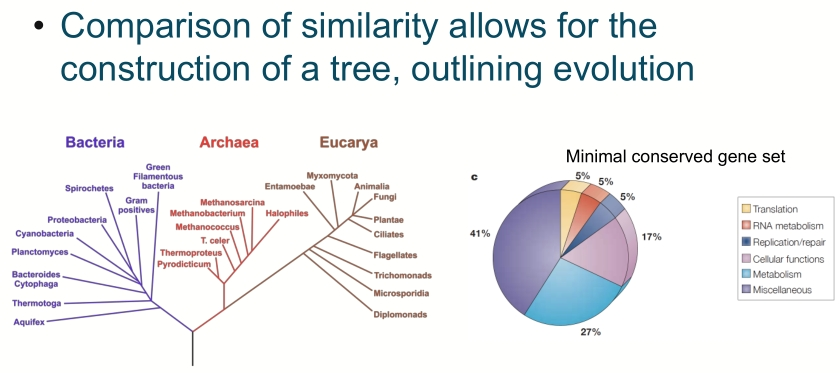
\includegraphics[width=0.9\textwidth]{Phylogeny}
\end{figure}

\begin{figure}[H]
	\caption{Horizontal gene transfer complicates things!}\label{fig:PhylogenyHorizontal} 
	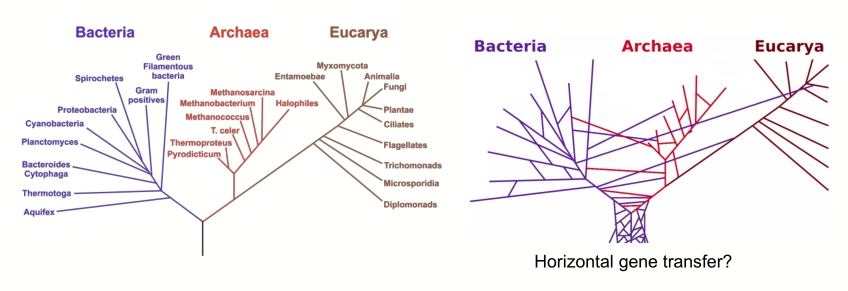
\includegraphics[width=0.9\textwidth]{PhylogenyHorizontal}
\end{figure}

\section{Selection Theory}
Chris Kempes

\subsection{Quasispecies equation}
\begin{itemize}
	\item How do we think about evolution in a simple, mathematical way?
	\item Start with binary Genome. One string can change into another via point mutations.
\end{itemize}


\begin{figure}[H]
	\caption{Topology of genome -- point mutations represent edges}\label{fig:GenomeTopology} 
	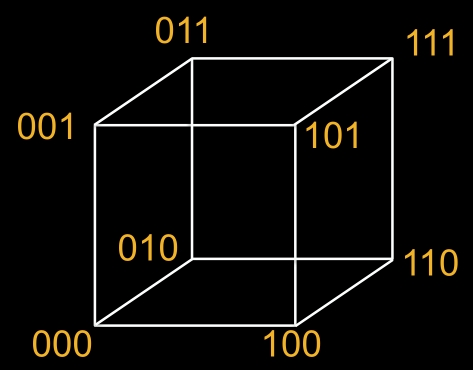
\includegraphics[width=0.9\textwidth]{GenomeTopology}
\end{figure}

\begin{figure}[H]
	\caption{Fitness Landscape, showing maximum fitness.}\label{fig:FitnessLandscape} 
	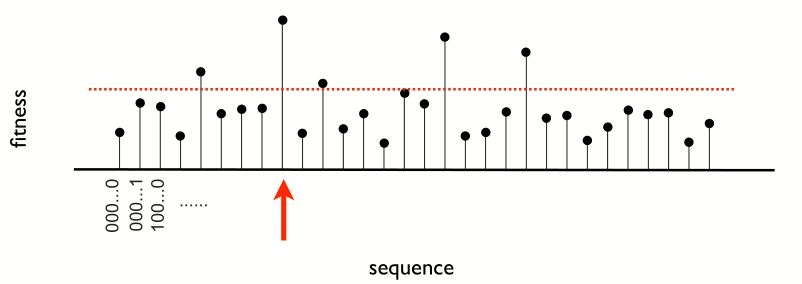
\includegraphics[width=0.9\textwidth]{FitnessLandscape}
\end{figure}

Introduce \emph{Quasispecies equation}.
\begin{align*}
\dot x_i =& f_i x_i - \phi x_i \text{, where $x_i$ is frequency of sequence $i$, $f_i$ is fitness, $\phi$ is death term.}\\
\sum_{i=1}^{n} \dot x_i =& 0 \text{, assume constant population}\\
\sum_{i=1}^{n} f_i - \phi \sum_{i=1}^{n} x_i =& 0\\
\phi =& \sum_{i=1}^{n}x_i f_i\text{, since $\sum_{i=1}^{n}x_i = 1$}
\end{align*}
Hence $\phi$ is \emph{average fitness}. But this leaves out \emph{mutation!} Include $q_{ij}$, the probability of mutation from $i$ to $j$.
\begin{align*}
\dot x_i =& \sum_{j=1}^{n} f_j q_{ij}x_j - \phi x_i\text{, full quasispecies equation} 
\end{align*}

NB. See Figure \ref{fig:GenomeTopology} - point mutations much more likely than 2-point, etc.

\subsection{What are the basic ways in which we think about evolution?}

\begin{itemize}
	\item How do we generalize evolution?
	\item How do we use this to think about origins of life? 
\end{itemize}

\begin{figure}[H]
	\caption{Simplify to \emph{Master Sequence}, $f_0$ with all less fit sequences lumped as $f_1$.}\label{fig:SteadyStateSolution} 
	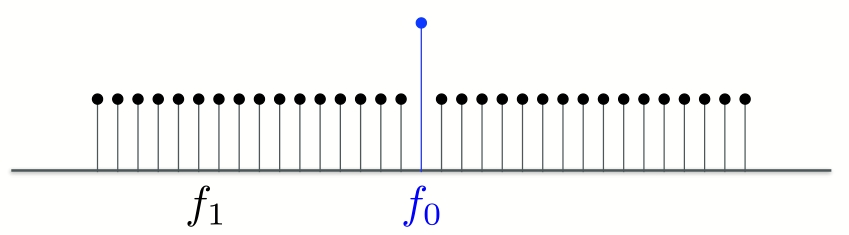
\includegraphics[width=0.9\textwidth]{SteadyStateSolution}
\end{figure}

\begin{align*}
\dot x_i =& \sum_{j=1}^{n} f_j q_{ij}x_j - \phi x_i\\
f_0 >&1, f_1 = 1\\
q_{00} =& (1-u)^L \triangleq q\text{, where $u$ is mutation rate, $L$ = length of genome}\\
q_{01} =& 1-q\\
q_{11} =& 1\text{, $L$ is large, so 1$\rightarrow$1} \\
q_{10} =& 0\text{, $1\nrightarrow0$}\\
\phi =& \sum_{i=1}^{n}x_i f_i\\
\text{Whence,}\\
\dot{x_0}=&f_0 q x_0 - \phi x_0\text{,}\\
\dot{x_1}=&f_0 (1-q) x_0 + x_1 -\phi x_1\text{, and}\\
\phi =& f_0 x_0 + x_1 \text{. But} \\
x_0 + x_1 =& 1\text{, so we have}\\
\dot{x_0}=& x_0 \big[f_0 q -1 - x_0 (f_0 - 1)\big]
\end{align*}
Now we can look for a steady state solution:
\begin{align*}
x_0^* =& \frac{f_0 q - 1}{f_0 - 1}\text{, se we need}\\
f_0q >& 1 \text{, if the master sequence is to persist. I.e.}\\
u <& log(f_0)\\
log(f_0) >& -L log(1-u)\text{. Now we assume $L<<1$, and find}\\
u <& \frac{log(f_0)}{L}\text{, which is known as the \emph{Error Threshold.}} 
\end{align*}
The Error Threshold is the \emph{maximum mutation rate that allows for adaptive evolution!} NB: it is more sensitive to $L$ than to $f_0$.

\subsection{Quasispecies and Error Catastrophe}

Michael Lachmann

We look at growth of types, e.g.:
\begin{itemize}
	\item Genome in population
	\item Molecule in test-tube.
\end{itemize}

\begin{align*}
\vec{x}^{\,t} =& W M \vec{x}\text{, where M represents mutations, W growth, e.g.}\\
M =& \begin{bmatrix}
1-\mu & 0\\
\mu& 1
\end{bmatrix}&
\end{align*}
Let us diagonalize WM
\begin{align*}
WM =& VDV^{-1}\\
(WM)^t =& V D^t V^{-1}
\end{align*}
So $D^t$ is dominated by its largest eigenvalue.

Figures \ref{fig:ErrorCatastrophe1} and \ref{fig:ErrorCatastrophe2} show that master sequence lost if mutation rate is too high. 
\begin{figure}[H]
	\caption{Hamming Distance.}\label{fig:ErrorCatastrophe1} 
	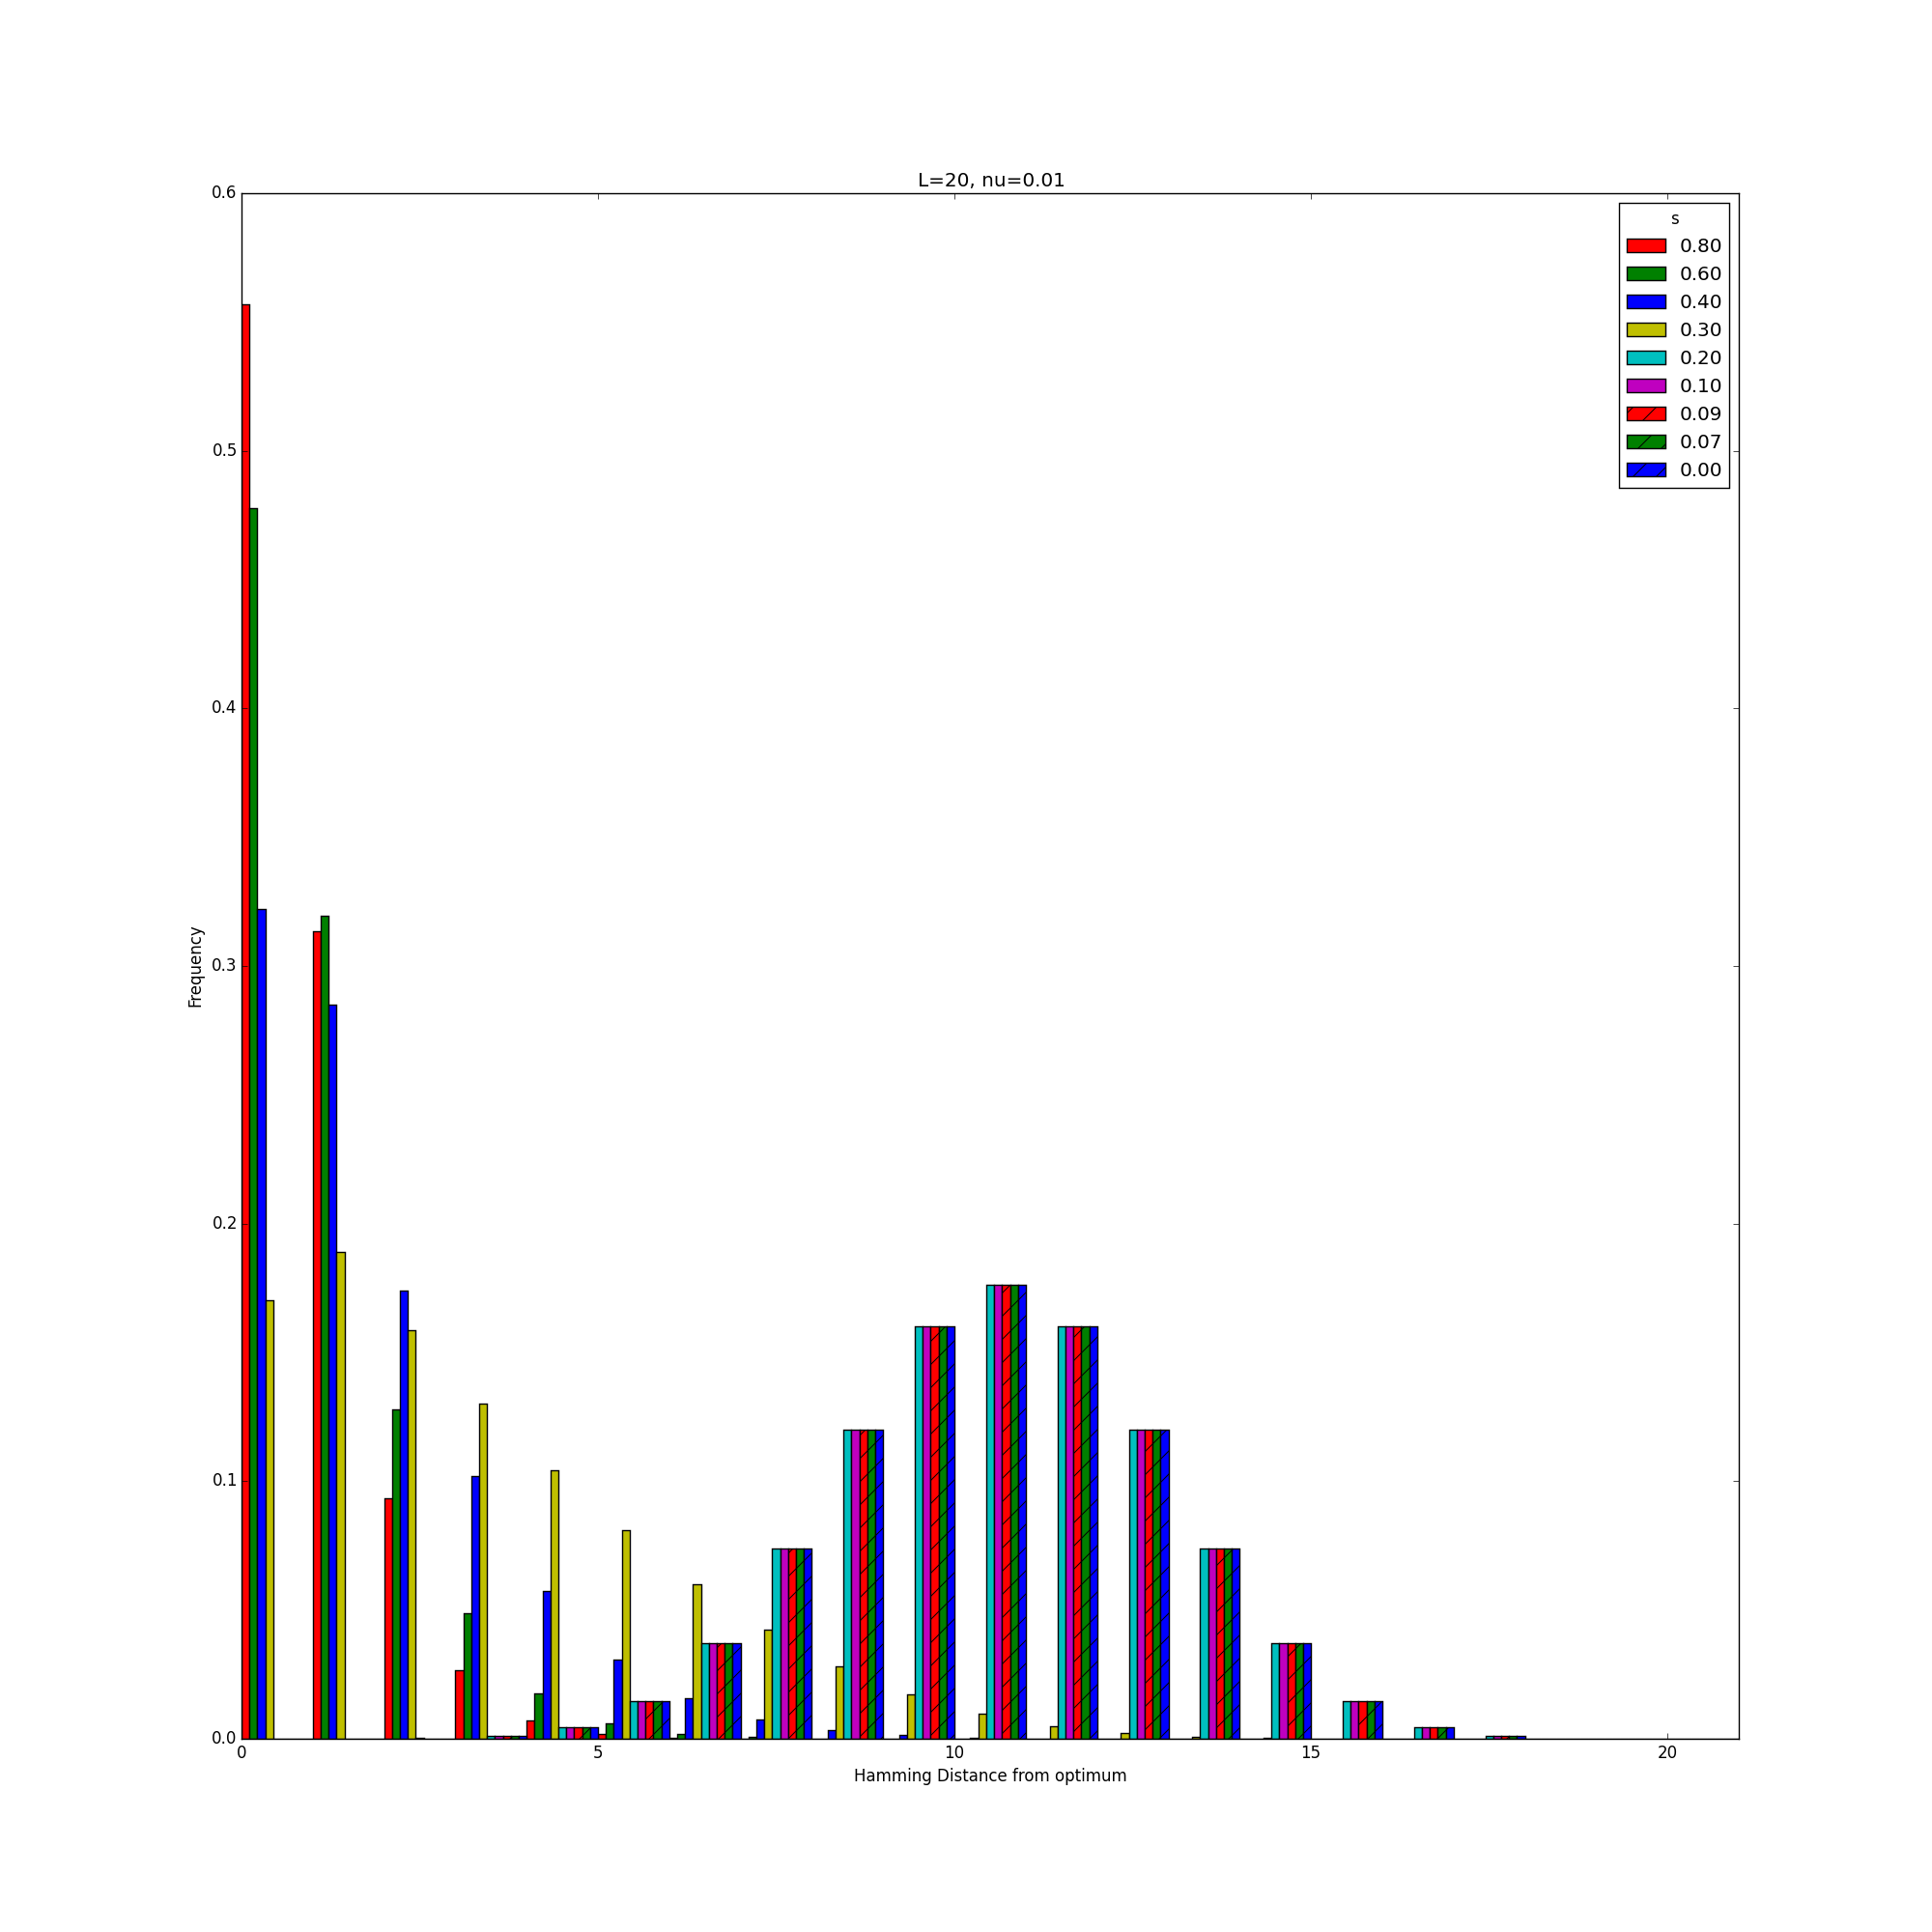
\includegraphics[width=0.9\textwidth]{ErrorCatastrophe1}
\end{figure}
\begin{figure}[H]
	\caption{Error Catastrophe.}\label{fig:ErrorCatastrophe2} 
	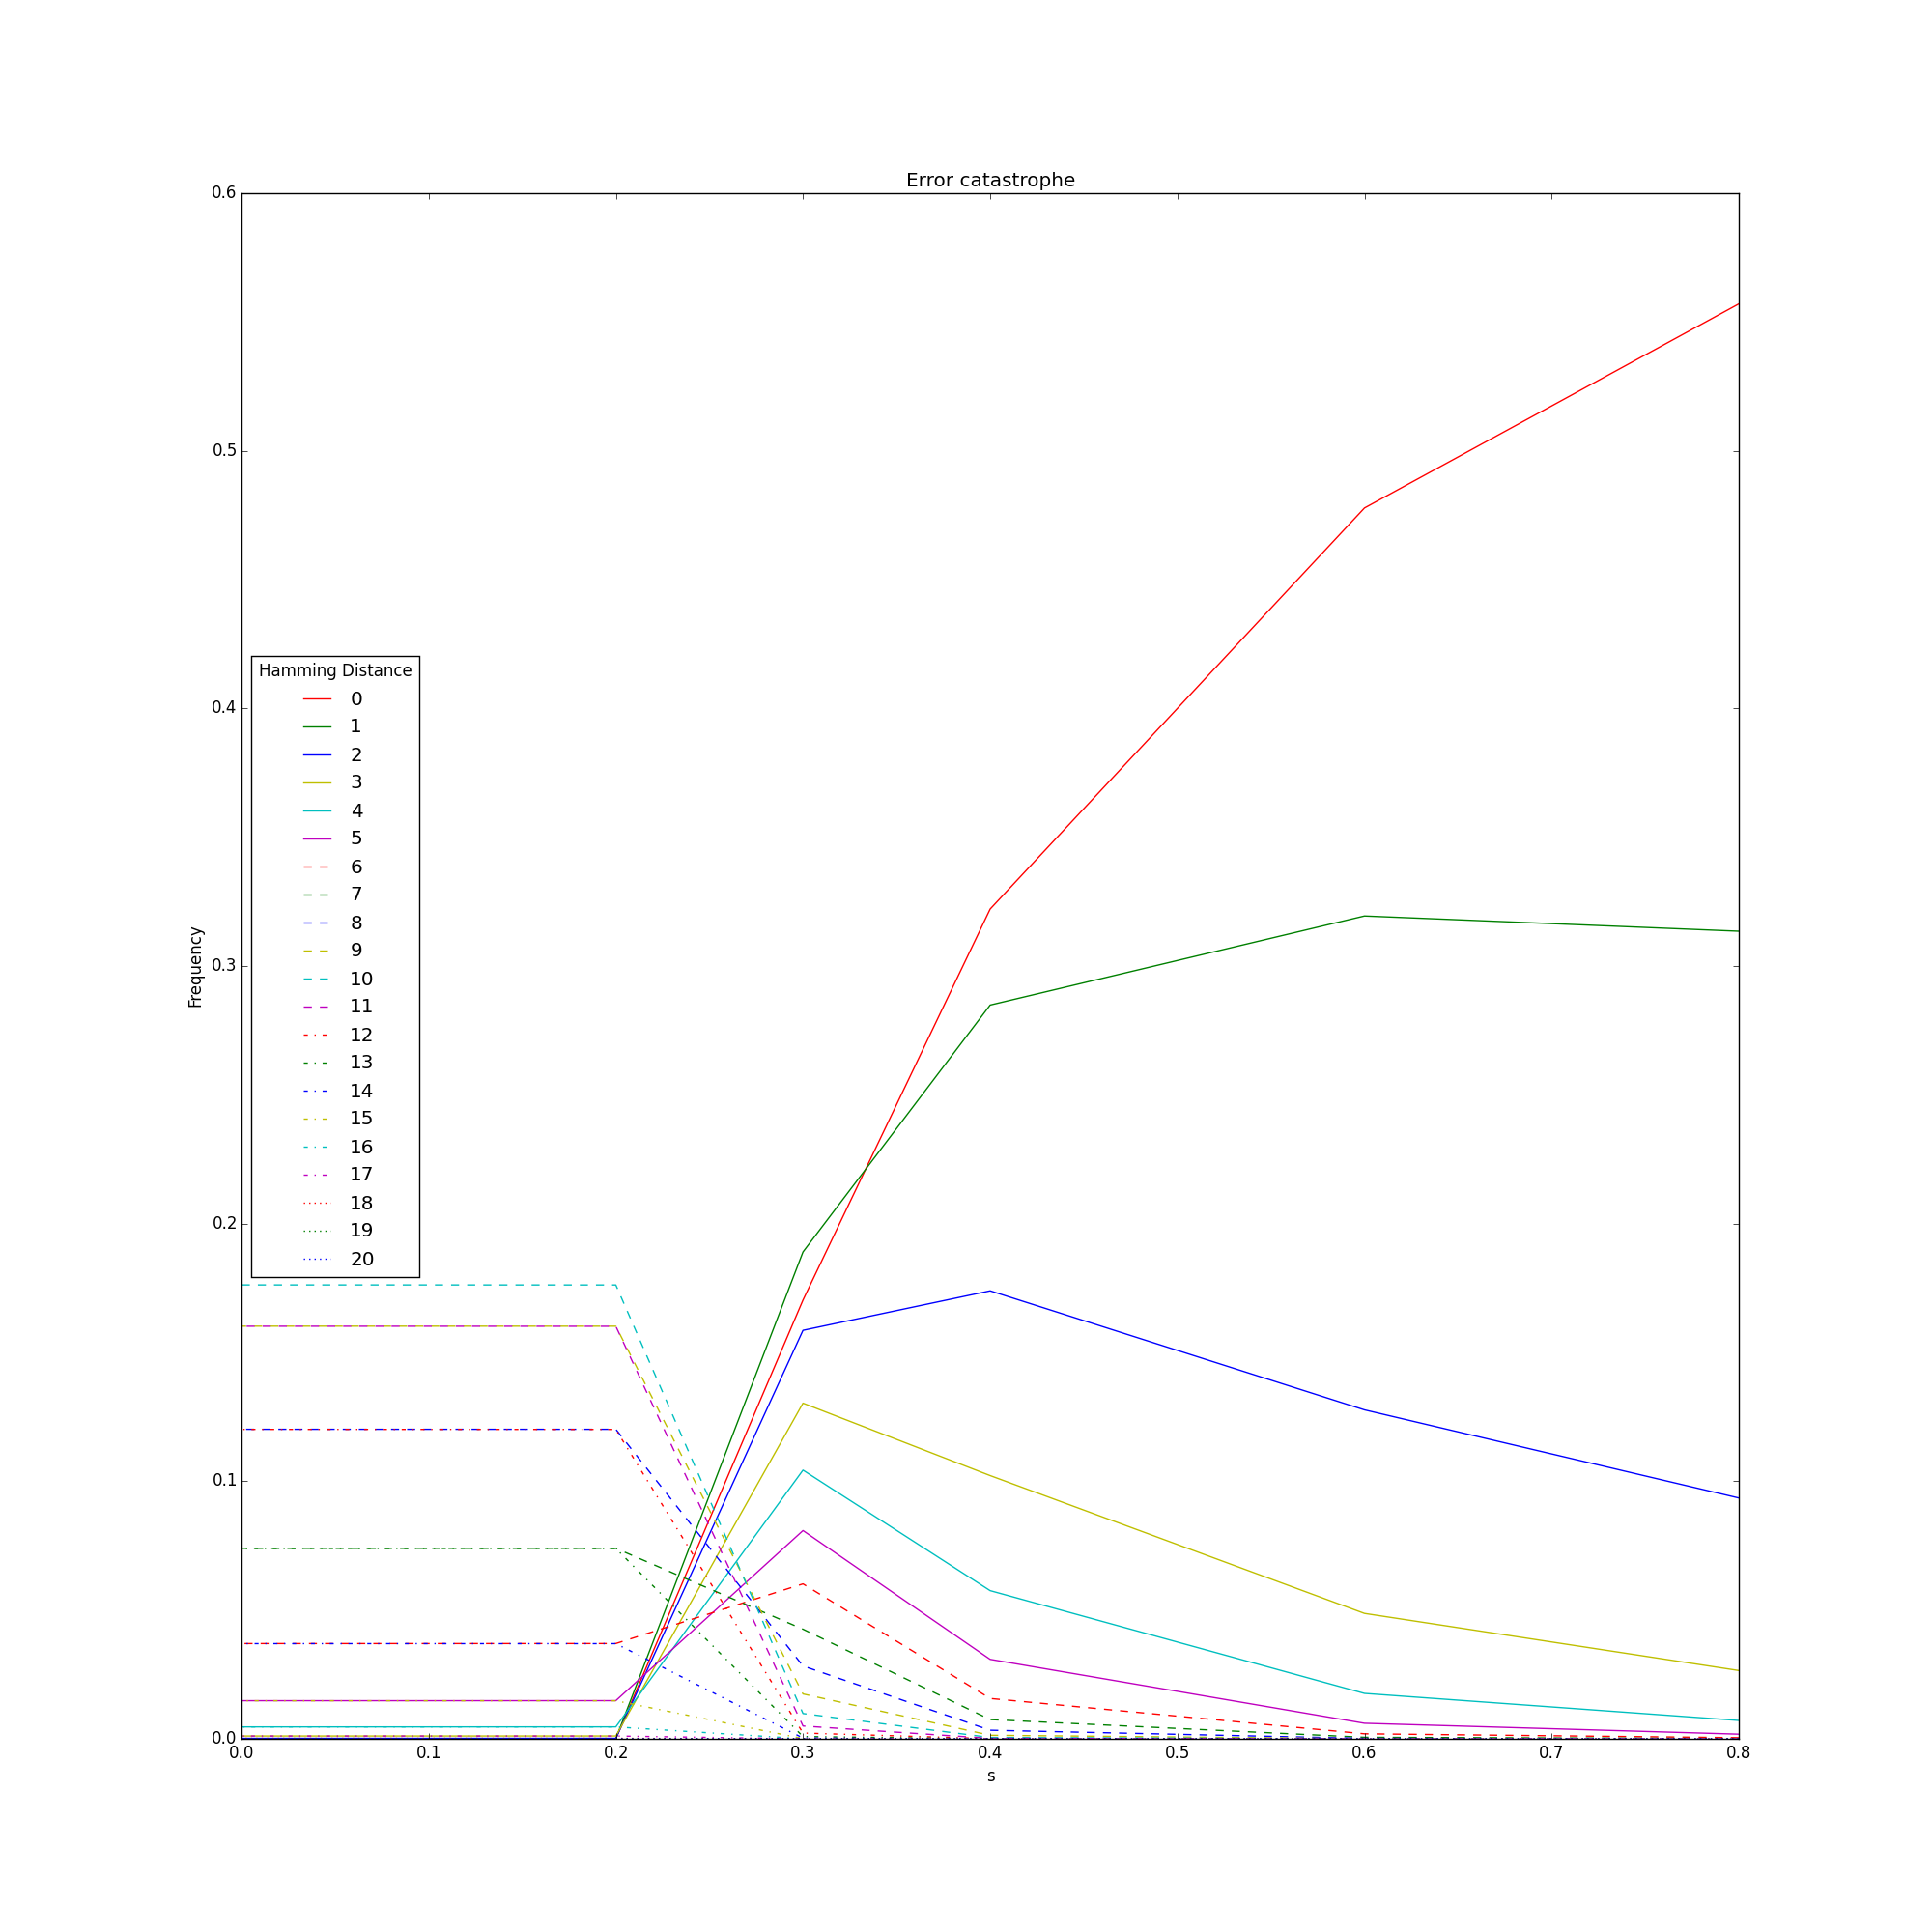
\includegraphics[width=0.9\textwidth]{ErrorCatastrophe2}
\end{figure}


See \cite{eigen1978hypercycle}, \cite{eigen1988molecular}, \cite{eigen2002error}, \cite{crotty2001rna}, and \cite{stadtler2002fitness_landscapes}.


% end of text 

% glossary: may need command makeglossaries.exe origins1
\printglossaries

% bibliography goes here
 
\bibliographystyle{unsrt}
\addcontentsline{toc}{section}{Bibliography}
\bibliography{origins}

\end{document}
